% EE Thesis/Dissertation
% Please see http://ee.tamu.edu/~tex for information about EE Thesis.

\documentclass[a4paper]{aitthesis}

\usepackage{graphicx}
\usepackage{latexsym}
\usepackage{amssymb,amsthm,amsmath}
\usepackage[notocbib]{apacite}

\AtBeginDocument{%
\renewcommand{\BBAY}{, }%% punctuation between authors and year
}

\usepackage{verbatim}
\usepackage{multirow}
\usepackage{bm}
\usepackage{url}
\usepackage{algorithm}
\usepackage{algcompatible}
\usepackage{placeins}
\usepackage{times}
\usepackage{array}

\usepackage[caption=false,font=footnotesize]{subfig}

\newcommand{\oops}[1]{\bf{#1}}
\newcommand{\ga}{\bar{\gamma}}
\newcommand{\myint}{\int_0^{\infty}}
\renewcommand{\vec}[1]{\mathbf{#1}}
\newcommand{\mat}[1]{\mathrm{#1}}
\newcommand{\todo}[1]{\arraybackslash{{TODO: #1}}}

\newcommand{\vectornorm}[1]{\left|\left|#1\right|\right|}

\newcommand{\ten}[1]{\mathcal{#1}}
\newcommand{\crossmat}[1]{\begin{bmatrix} #1 \end{bmatrix}_{\times}}
\newcommand{\class}[1]{{\cal C}_{#1}}
\def\Rset{\mathbb{R}}
\def\Pset{\mathbb{P}}
\DeclareMathOperator*{\argmax}{argmax}
\DeclareMathOperator*{\argmin}{argmin}
\DeclareMathOperator*{\sign}{sign}
\def\norm{\mbox{$\cal{N}$}}

\newcommand\parms{\vec{\lambda}}
\newcommand\oldparms{\parms^{\text{old}}}

\def\short{1}

\begin{document}

\pagenumbering{roman}
\pagestyle{plain}
%==========================================================
%======================  FRONT STUFF ======================
%==========================================================

%======================= Cover Page =======================
%\begin{document}
\newpage
\pagestyle{plain}
\pagenumbering{roman}
\setcounter{page}{1}
\addcontentsline{toc}{section}{Title Page}
%\setlength{\footskip}{-15mm}
\setlength{\textheight}{230mm}
\setlength{\voffset}{10mm}
\vskip -5em

\begin{center}
{ 
  \singlespace \uppercase{\bf Multi-Agent Aerial Mapping Using Structure from Motion and Wireless Mesh Networks} \par
}
\vskip 2em
{
  \lineskip 1.5em
  \begin{tabular}[t]{c} by\\ \\ Raunak Mukhia
  \end{tabular}\par
}
%\vskip 5.6em

\vskip 3.5em
\singlespace A thesis submitted in partial fulfillment of the
requirements for the\\ degree of Master of Engineering in\\ 
Computer Science 

%	\vskip 5em
\vskip 0.5em
{
  \singlespace
  \begin{center}
    \begin{tabular}{rl}
      \\[-1em]
      Examination Committee: & Dr.\ Matthew N. Dailey (Chairperson) \\[-0.8em]
                             & Dr.\ Adisorn Lertsinsrubtavee \\[-0.8em]
                             & Dr.\ Mongkol Ekpanyapong \\\\

% UNCOMMENT THE LINES BELOW IF YOU HAVE THE EXTERNAL EXAMINER.
%      External Examiner:     & Prof.\ YOUR EXTERNAL EXAMINER \\[-0.8em]
%                             & Dept.\ of Electrical and Computer Engineering \\[-0.8em]
%                             & McGill University, Canada \\\\
		
      Nationality:     & Indian \\[-0.8em]
      Previous Degree: & Bachelor of Technology in Computer Science and Engineering \\[-0.8em]
                       & Sikkim Manipal Institute of Technology, India\\[-0.8em]
      \\
      %Scholarship Donor: &\\[-0.8em]
      \\
    \end{tabular}
  \end{center}

  \vskip 3.0em
  \centerline{}
  \vskip 2em
}
\end{center}
\begin{center}
  \singlespace Asian Institute of Technology\\ School of Engineering
                  and Technology\\ Thailand\\ December 2020
\end{center}
\vfill

%====================== ACKNOWLEDGEMENTS ======================
\newpage
\pagestyle{plain}
\addcontentsline{toc}{section}{Acknowledgments}
\onecolumn % Single-column.
\if@twoside\else\raggedbottom\fi % Ragged bottom unless twoside option.
\setlength{\footskip}{8mm}
\begin{center}
{
  \large \bf Acknowledgments\\ \vskip 1em
}
\vskip 1em
\end{center}
\singlespace
\doublespace
\hspace{8.5mm}
\vspace{-1em}

Write your touching message here..

%====================== ABSTRACT ======================
\newpage
\pagestyle{plain}
\addcontentsline{toc}{section}{Abstract}
\onecolumn % Single-column.
\if@twoside\else\raggedbottom\fi % Ragged bottom unless twoside option.

\setlength{\footskip}{8mm}

\begin{center}
{\large \bf Abstract \\ \vskip 1em}
\vskip 1em
\end{center}
\singlespace
\doublespace
\hspace{8.5mm}
\vspace{-1em}

Abstract here..

\setlength{\parskip}{0pt} 
%======================= Table of Contents =========================
\newpage
\addcontentsline{toc}{section}{Table of Contents}
\tableofcontents

% Page 2 begins

%===================== List of Figures ======================
\newpage
\addcontentsline{toc}{section}{List of Figures}
\listoffigures

%\clearpage     % \clearpage ends the page, and also dumps out all floats.
%\end{document} % Floats are things like tables and figures.

%\clearpage     % \clearpage ends the page, and also dumps out all floats.

% %===================== List of Tables ======================
\newpage
\addcontentsline{toc}{section}{List of Tables}
\listoftables

% %\clearpage     % \clearpage ends the page, and also dumps out all floats.
% %\end{document} % Floats are things like tables and figures.

%\clearpage     % \clearpage ends the page, and also dumps out all floats.

\setlength{\parskip}{12pt}


\small

\pagenumbering{arabic}
\setlength{\headheight}{12pt}
\pagestyle{plain}

\setlength{\footskip}{8mm}

\chapter{Introduction}

\textit{  }

\section{Overview}

The availability and financial accessibility of unmanned aerial vehicles (UAVs) have made them more widespread, finding application in a wide range of civilian activities. Multi-rotors are used for recreational flying, research, cinematography, disaster observation, logistics, agriculture,  public safety, construction, surveillance, and environmental protection, amongst other things. 

A cluster of inexpensive autonomous multi-rotors connected through a wireless mesh network that can be deployed in a post-disaster situation can help avoid dangerous situations faced by ground-based human observers in such scenarios. The drones can do aerial mapping quickly, as they can coordinate so that one drone does not need to visit locations already visited by other drones in the cluster. The range of the cluster can also be large, as each drone will act as a wireless mesh access point. Furthermore, each drone can act as an access point to provide connectivity in the area.  

For aerial mapping, drones can be fitted with an array of sensors such as ultrasonic, infrared, multi-array laser sensors, and RGB-D cameras. Systems with many sensors have integration complexities and may suffer from weight constraints, reduced battery lifetime, and high cost. Monocular visual SLAM provides a low cost, light weight, simple alternative to sensor-intensive approaches. 

This study proposes a system of a cluster of autonomous drones, each being a node in a wireless mesh network, that performs coordinated exploratory aerial mapping using vSLAM.

\section{Problem Statement}


An inexpensive cluster of UAVs providing autonomous coordinated aerial mapping after a disaster can be a valuable asset for disaster observation and public safety, without posing risk for ground-based surveillance personnel. A wireless mesh network can also be an inexpensive solution when communication infrastructure like cellular data service is dysfunctional. The number of drones in the system is proportional to the desired range of the mesh network, because each drone can be a mesh node. UAVs providing emergency network services using mesh networks in disaster-struck areas is an active research area as discussed by  \shortciteA{dronewirelessmeshnetworkchand}. \shortciteA{Sabino_2018} discusses the optimal placement of UAVs' in a mesh network. A survey by \shortciteA{ZOU2019461} discusses the various multi-agent vSLAM methods available. \shortciteA{multiuavnetwork} uses mesh networks and SLAM with multiple UAVs but they control the UAVs manually, the SLAM results are not merged into a global map, and they do not implement coordination and autonomous path planning within the constraints of a mesh network.

Monocular vSLAM requires only one camera, but it suffers from issues of map initialization and scale ambiguity. That is, the size of the environment as mapped will not be to scale. Integrating accelerometer and gyroscope measurements can help determine an approximate scale.


\section{Objectives}


The main objective of this thesis is to improve on the state of the art in mapping disaster-stricken areas by implementing a method for autonomous multi-agent exploration and coordinated aerial mapping with vSLAM. The focus of this study is to map a disaster-struck area with the possibility of damage to communication infrastructure; therefore, the system will use a wireless mesh network for internal communication, with each agent working as a mesh node. The objectives can be decomposed into the following specific tasks:
\begin{itemize}
	\item Design and implement a wireless mesh network with each drone as a mesh node. As the drones are fast-moving agents, this will require study and implementation of solutions to maintain a reliable network with a usable quality of service, despite constant topology changes.
	\item Implement monocular vSLAM to generate an aerial map of the area under surveillance, and merge the point clouds generated by different agents into a single global map.
	\item Design and implement an autonomous exploration and coordination system for the agents that operates within the restriction of the range of the wireless mesh network. This system should also maximize the range of the surveillance, by finding an optimal arrangement of the agents over time.
\end{itemize}

\todo{ Flight time restrictions }




\section{Limitations and Scope}

Some text ...

\section{Thesis Outline}

I organize the rest of this dissertation as follows.

In Chapter \ref{ch:literature-review}, I describe the literature review.

In Chapter \ref{ch:methodology}, I propose my methodology.

In Chapter \ref{ch:results}, I present the experimental results.

Finally, in Chapter \ref{ch:conclusion}, I conclude my thesis.

\FloatBarrier

\setlength{\footskip}{8mm}

\chapter{Literature Review} 
\label{ch:literature-review}

\textit{This chapter begins with a review of the functional architecture of autonomous driving systems, coordinate systems, the PixHawk, and ROS coordinate conventions.} 

\section{Software Architecture of Autonomous Driving Vehicles}
\label{section-name-in-literature-review}

\shortciteA{sbehere16t} splits the major components of the motion control part of autonomous driving systems into three main categories as shown in Figure \ref{fig:fav_automonous}. These categories are

\begin{itemize}
	\item Perception of the external environment in which the vehicle operates
	\item Decision making and control of vehicle motion with respect to the external environment that is perceived
	\item Vehicle platform manipulation, which deals mostly with sensing, control, and actuation of the vehicle, with the intention of achieving the desired motion.
\end {itemize}

Each category can be further broken down into several components. I describe each component in more details in the following sections.

\subsection{Perception}

Sensing components sense the state of the vehicle and the state of the environment in which the vehicle operates. The sensor fusion component considers multiple sources of information to construct a hypothesis or belief about the state of the environment. The localization component determines the location of the vehicle with respect to a global map. The semantic understanding component processes the sensor input and derives meaningful information from it. The world model component holds the current estimate of the state of the external environment.

\subsection{Decision and Control}
The trajectory generation component repeatedly generates a set of obstacle-free trajectories in the world coordinate system and picks an optimal trajectory from the set. Energy management components deal with energy management of the vehicle. Diagnosis and fault management monitors the state of the overall system and its components. Reactive control components are used for immediate responses to unanticipated stimuli from the environment. The vehicle platform abstraction component refers to a minimal model of the vehicle platform. 

\subsection{Vehicle Platform Manipulation}

The platform stabilization component's task is to keep the vehicle platform in a controllable state during operation. Trajectory execution components are responsible for executing the trajectory generated by the decision and control component. 

\begin{figure}
	\centering
	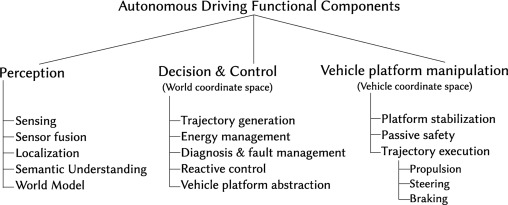
\includegraphics[width=5in]{figures/literature/fav_autonomous_driving}
	\caption[FAV of Antonomous Driving System.]{\small 
		Functional architecture of an autonomous driving system. Reprinted from Behere (2016). }
	\label{fig:fav_automonous}
\end{figure}

\section{Coordinate Systems}

In this section I describe the different coordinate system conventions in use in robotic applications. 
	
\subsection{Earth Centric, Earth Fixed}

The earth-centered earth-fixed (ECEF) coordinate system, rotates with the Earth and has its origin at the center of the Earth. Refer to Figure~\ref{fig:coordinatesystem} (a) for a visualization. ECEF follows the right handed coordinate system convention. \shortciteA{coordinatesystem} describes ECEF as follows.

\begin{itemize}
	\item The origin is at the center of mass of the Earth, a point close to the Earth's center.
	\item The Z axis is on the line between the magnetic north and south poles, with positive values increasing northward (but not exactly coinciding with the Earth's rotational axis).
	\item The X and Y axes lie in the plane of the equator.
	\item The X axis passes through the point on the equator from 180 degrees longitude (negative) to the prime meridian (0 degrees longitude, positive).
	\item The Y axis passes through the point at 90 degrees west longitude along the equator (negative) to 90 degrees east along the equator (positive).
\end{itemize}

\subsection{World Geodetic System}
The World Geodetic System is a standard system used in GPS, cartography and geodesy. The latest revision is WGS 1984 (WGS 84) that was established and is maintained by the United States National Geospatial-Intelligence Agency. It was last revised in 2004. The World Geodetic System 1984 (WGS 84) is one of the best global geodetic reference system for the Earth available presently. The datum (ellipsoid) defined by WGS 84 is generally used to convert the GPS latitutes and longitude to the UTM coordinate system.

\subsection{Universal Transverse Mercator Geopraphic Coordinate System}
The Universal Transverse Mercator (UTM) is a coordinate system that divided the earth into 60 zones. Each zone is a plane with its own x and y coordinates in meters. It ignores altitude and treats the earth as a perfect ellipsiod. A UTM coordinate has:

\begin{itemize}
        \item A zone number.
        \item A hemisphere (N/S).
        \item An easting (X coordinate).
        \item A northing (Y coordinate)
\end{itemize}

A coordinate 14.08057584 \degree N, 100.61284553 \degree E in latitude and longitude is represented as 47 N 674132 1557234 in UTM.

\subsection{Local tangent plane}

In the local tangent plane coordinate system, a position on the earth is fixed about the origin. There are two conventions as shown in Figure~\ref{fig:coordinatesystem} (b).

\begin{itemize}
	\item X=East, Y=North, Z=Up (ENU).
	\item X=North, Y=East, Z=Down (NED), which is commonly used in aviation, as the objects of interest usually lie before an aircraft (down or positive Z).
\end{itemize}

\begin{figure}%
	\centering
	\subfloat []{{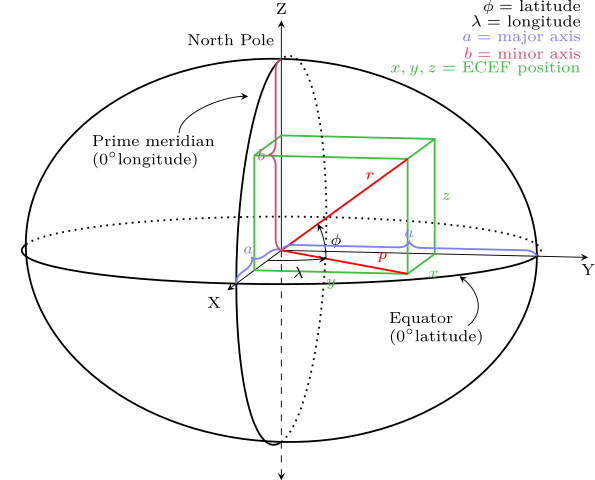
\includegraphics[width=3in]{figures/literature/ECEF}}}%
	\subfloat []{{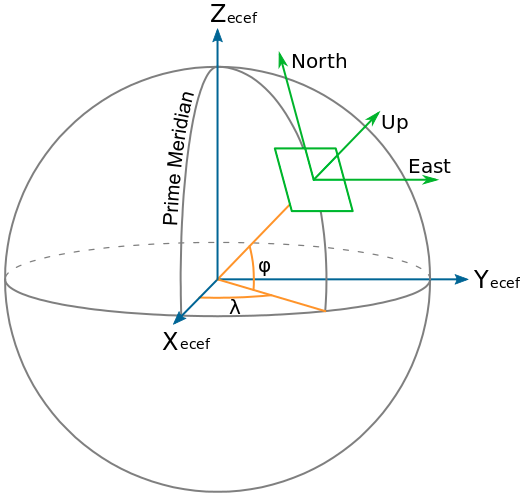
\includegraphics[width=3in]{figures/literature/ENU_NED}}}%
	\caption[ECEF coordinate system]{\small Coordinate systems. (a) Earth centric, earth fixed (ECEF) coordinate system. (b) Local tangent plane coordinate systems. Reprinted from Krishnavedala. 
	}%
	\label{fig:coordinatesystem}%
\end{figure}

\subsection{PixHawk and ROS coordinate systems}

PixHawk follows the NED convention, whereas ROS follows the ENU convention. The conversion between these different conventions is handled automatically by MAVROS. To translate air-frame related data, a rotation of $180^{\circ}$ degrees is applied about the roll (X) axis. For local data, a $180^{\circ}$ rotation is applied about the roll (X) and $90^{\circ}$ rotation is applied about the yaw (Z) axes.

It is good practice in ROS to set up reference frames as described by \shortciteA{rosrefframes}, shown in Figure \ref{fig:rosrefframes}.

\begin{itemize}
	\item The coordinate frame called base\_link is rigidly attached to the mobile robot base. It can be attached in any arbitrary position or orientation.
	\item The coordinate frame called odom is a world-fixed frame. The pose of a robot is continuous in this frame, but it can drift over time.
	\item The coordinate frame called map is a world fixed frame, with Z-axis pointing upwards. 
	\item The coordinate frame called earth is the origin of the ECEF frame.
\end{itemize}

\begin{figure}
	\centering
	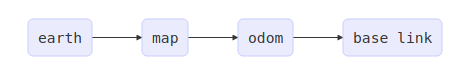
\includegraphics[width=5in]{figures/literature/ros_rel_frames}
	\caption[Relation between ROS frames]{\small 
	Relationship between ROS frames. Reprinted from \shortciteA{rosrefframes}. }
	\label{fig:rosrefframes}
\end{figure}

\section{Wireless Mesh Network}

A wireless mesh network's (WMN) consists of two types of nodes, mesh routers and mesh clients. Mesh routers form the mesh backbone for mesh clients. Every node in the mesh has the capability to route packets forward for other nodes if the packet destination is not in direct wireless transmission range. Mesh routers provide functionality as bridge/gateway that enables the WMN to integrate with other networks such as cellular, ad-hoc and ethernet. In a wireless mesh network, all the participating nodes automatically establish and maintain mesh connectivity and are in effect dynamically self-organized and self-configured. WMN can be rapidly deployed where there is no network coverage and has the potential for application in disaster management.

\subsection{WMN Network Architecture}

A wireless mesh network has two types of nodes, mesh routers and mesh clients. Mesh routers can have multiple networking interfaces to provide bridge/gateway functionality to the mesh network and have additional routing functions to support mesh networking. Mesh routers can be built on similar hardware platform as a conventional wireless router. Mesh routers can be build based upon embedded systems and general-purpose computer systems. Mesh clients have capability for mesh networking and can also work as a mesh router, nevertheless they lack bridge/gateway function and usually have only one wireless interface.


The architecture of WMNs can be classified into three types based upon the composition of mesh routers and clients.

\begin{itemize}
	\item \textit{Infrastructure/Backbone WMNs.}
	In this architecture mesh routers form an infrastructure for clients that connect to them. The mesh routers automatically establish and maintain links between themselves and provide gateway functionality to connect the mesh network to other networks and the internet. 
	
	\item \textit{Client WMNs.} In this architecture, mesh routers are not required for maintaining a mesh network. Mesh clients provide peer-to-peer networking, performing routing and configuration management. A packet may reach the destination node through multiples hops through client nodes.
	  
	\item \textit{Hybrid WMNs.} In this architecture, mesh routers provide infrastructure backbone with access to other networks. Client nodes can connect to the mesh network through meshing with other clients, as well as through mesh routers. This in effect, is a combination of infrastructure and client WMNs, and provides increased connectivity and coverage.
\end{itemize}

\subsection{Features of WMNs}

WMNs have redundant nodes and can provide high level of fault tolerance and robustness. If the case of link failure, the mesh network can adapt and reroute the data. Using multi-hop strategies, the coverage range can be increased, as intermediate router and clients can relay packets between hosts which do not have a direct line of sight. WMNs can be rapidly deployed with less maintenance because of self-forming, self-healing and self-organization capability. They are compatible with ad-hoc wireless clients.


\subsection{Routing Protocols for WMNs}

WMNs has redundant and mobile clients, hence, the routing protocols should find and maintain routes between the source and destination nodes by detecting and responding to changes in network topology. Ideally routing protocols should maximize the capacity of the network and minimize the packet delivery delays by creating and selecting efficient routes between nodes.

Wireless mesh routing protocols can be classified into three categories:

\begin{itemize}
	\item \textit{Proactive Routing Protocol.} Proactive routing protocols build and maintain the routing table by sharing routing data among nodes at periodic intervals. It selects the route from the routing table while forwarding packets from one node to the other. Optimized Link State Routing Protocol (OLSR) and Better Approach to Mobile Ad-hoc Networks (BATMAN) falls under this category.
	\item \textit{Reactive Routing Protocol.}  Reactive routing protocols searches the route from source to destination node on demand as it is required. Examples of this category are Ad Hoc On-Demand Distance Vector Protocol (AODV) and Dynamic Source Routing Protocol (DSR).
	\item \textit{Hybrid Routing Protocol.} Hybrid Routing Protocol uses both reactive and proactive routing strategies depending upon the environment. As a reactive routing protocol, it will provide the path on demand, based on up-to-date information. Examples of hybrid routing protocols are ZRP (zone routing protocol), HSLS (hazy sighted link state routing protocol).
\end{itemize}

\subsubsection{Comparision of Routing Protocols}

\shortciteA{Mbarushimana2007} does a comparative study between the performance of reactive (AODV and DSR) and proactive (OSLR) protocols. They run simulations for 1000 seconds, considering four different scenerios, namely, workload, number of flows, number of nodes in the network, and node movement speed. The performance of the three routing protocols is measured based on throughput, goodput, routing load and end-to-end delay. They come to the conclusion that OSLR shows the best performance in terms of data delivery ratio and end-to-end delay, and provide insight that network layer tends to drop more packets while reactive protocol is computing the route to the destination. In their study OSLR still outperforms the reactive routing protocols at higher speeds even though it has the highest routing overhead due to its exchange of periodic routing updates.

\shortciteA{Kulla2012} does a performance comparison of OSLR and BATMAN routing protocols in an indoor stairs environment of 5 floor building. They come to the conclusion that both the protocols perform well for one-hop and two-hop communication. The delay and packet loss increased after three hops for static node scenario and after two hops for moving node scenario. BATMAN performs better than OSLR for packet loss metrics because BATMAN buffers packets when routes are unstable. In general, OSLR protocol showed better performance than BATMAN protocol. OSLR shows better performance than BATMAN regarding the delay metrics, which is critical for realtime communication between a cluster of drones.

From these studies of performance comparisons OSLR seems to be the most suited to my use case, as:
\begin{itemize}
	\item Proactive protocols (OSLR) performs better than reactive protocols in terms of data delivery ratio and end-to-end delay.
	\item Reactive protocols tends to drop packets while they are computing the route.
	\item OSLR shows better performance than BATMAN for delay metrics.
	\item Latest information about the drones in the mesh network is more critical than stale information, which means OSLR with less delay is more suited to the use case of my study.
\end{itemize}

\subsection{Optimized Link State Routing Protocol}

Optimized Link State Routing Protocol (OSLR) belongs to the class of link state routing protocol, with optimization for mobile ad hoc networks.  It is a distributed protocol with no central agency that exchanges topology information with other node of the network periodically. Each node maintains a routing table, and is a proactive protocol. When data is to be sent, it refers to the routing table. The route to other nodes are maintained by each node proactively. 

HELLO message is used for link sensing, neighbor detection, and multipoint relay (MPR) selection. HELLO messages are not forwarded by the nodes. The nodes in OSLR use only selected nodes called multipoint relay (MPR) to re-transmit control messages, reducing overhead from control messages flooding the network. Each node in the network selects a set of nodes in its symmetric 1-hop neighborhood called MPR set of that node. Neighbors which do not belong to MPR set of the node receive and process broadcast messages but do not re-transmit it. If an interface of a node has at least one verified bi-directional link with an interface of another node, it is considered as its symmetric 1-hop neighbor. 

Topology Control (TC) message is used to disseminated topology information through the network, using optimized flooding through MPR mechanism. The TC messages distributed to each node is used to calculate routing table in each node.

If a node has multiple interfaces, it must announce, periodically, information describing its interface configuration to other nodes in the network. Multiple Interface Declaration (MID) message is flooded by such nodes using MPR mechanism in the network, and is used for routing table calculations.

Gateway/bridge nodes have non OSLR interfaces connected to external network such as the ethernet. Host and Network Association (HNA) message are periodically broadcasted by such nodes to register such routing information in the routing table.


The role of OSLR is not to forward data packets. It maintains the routing table in each node which is used by the system to perform network layer forwarding function.

\subsection{FANET}

Flying ad hoc network (FANET) is a specialized subset of mobile ad hoc network(MANET). FANET takes into consideration the challanges faced by MANET with flying UAVs as the mesh nodes. FANET can also be classified as a subset of Vehicular ad hoc network (VANET), where the mesh nodes are vehicles on the ground. The relation between MANET, VANET and FANET is given in figure \ref{fig:manet-vanet-and-fanet}.

\begin{figure}
	\centering
	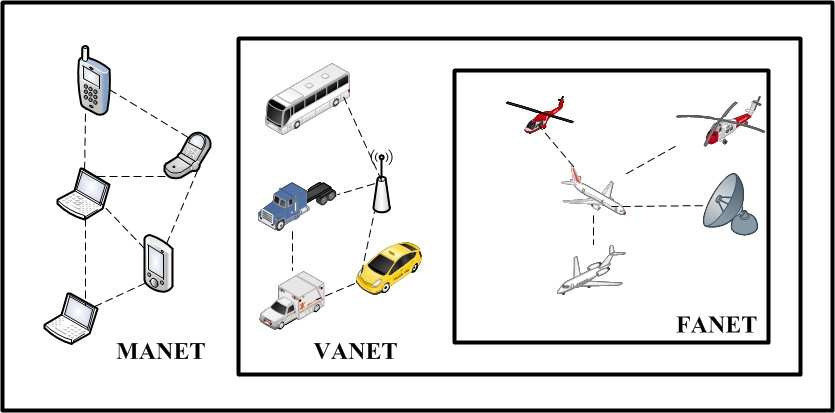
\includegraphics[width=5in]{figures/literature/MANET-VANET-and-FANET}
	\caption[MANET, VANET and FANET]{\small 
		MANET, VANET,and FANET Reprinted from \shortciteA{Tareque2015}. }
	\label{fig:manet-vanet-and-fanet}
\end{figure}

Surveys of FANET has been carried out by \shortciteA{Chriki2019} and \shortciteA{Tareque2015}. The challenges of FANET described can be summarized as follows:

\begin{itemize}
	\item \textit{Network topology change.} In FANET, rapidly moving UAVs changes the network topology more frequently.
	\item \textit{Node mobility.} UAVs have a higher degree of mobility than vehicles or people on ground. Node mobility issues can be considered as the most significant difference between FANET and other ad hoc networks.
	\item \textit{Node density.} Node density in FANET is lower than other MANETs. FANET nodes are spread across the sky. There are less number of average nodes in a unit area in FANET. 
	\item \textit{Radio propagation model.} MANET and VANET nodes are close to the ground and because of the environment, they may not have direct line of sight. FANET nodes are in the sky and for most cases have direct line of sight between the nodes.
	\item \textit{Power Consumption.} For large UAVs power consumption is not a significant factor when designing the FANET. However for small UAVs the power consumed by FANET must be taken into consideration.  
	\item \textit{Localization.} UAVs because of its higher mobility degree may have inaccurate GPS position information as compared to other MANETs.	
\end{itemize}

Routing protocols for FANET follows similar classification as WMNs and are as follows:

\begin{itemize} 
	\item \textit{Static protocols.} These protocols have fixed routing tables.
	\item \textit{Proactive protocols.} Updates the routing tables periodically.
	\item \textit{Reactive protocols.} Finds path to the destination node when data needs to be sent.
	\item \textit{Hybrid protocols.}  These use both reactive and proactive strategies when required. 
	\item \textit{Geographic based protocols.} These protocols use position information.
\end{itemize}

There are multiple optimization and extensions for OSLR specifically done to solve challenges for FANET. Some of them are:

\begin{itemize}
	\item \textit{DOLSR.} \shortciteA{Alshabtat2011} proposes Directional Optimized Link State Routing Protocol (DOLSR) which uses directional antenna and heuristic to minimize the number of MPRs. They show reduced end-to-end delay and enhanced overall throughout using DOLSR for FANET.
	\item \textit{P-OSLR.} \shortciteA{Rosati2013} proposes Predictive OSLR (P-OSLR) that uses GPS information to help the routing protocol. It take the relative speed between the nodes in account to calculated expected transmission count (ETX) metric. This metric is used by OSLR for link quality sensing. The show increased multi-hop reliability with minimum outage time as compared to OSLR in FANET environment.
	\item \textit{ML-OSLR.} \shortciteA{Zheng2014} proposes Mobility and Load aware OSLR (ML-OSLR) that introduces mobility and load aware algorithm in the routing protocol. ML-OLSR does not select high speed nodes as the MPR and avoid routing through high load, congested and high speed nodes to increase network stability. They show increased performance in packet delivery ratio and average end-to-end delay compared to OSLR with FANET based simulation.
\end{itemize}

\shortciteA{Singh2015} presents the application of OSLR to FANET under different mobility model of the nodes through simulation. He shows that the increase in speed of nodes decreases throughout, increases end to end delay and decreases packet delivery ratio for most mobility model. However for my study, the speed of the node are relatively low, and nodes spend most of their time waiting for other nodes to arrive to their waypoint and take picture, therefore I shall purse the use of generic OSLR for this thesis.


\section{Simulators}

An approximate imitation of a process or system's operation over time is known as simulation. A real-life or hypothetical situation modeled on a computer ro I how the system works is a computer simulation. Computer simulation can be a powerful tool to develop, investigate the behavior and save cost, by providing a means to virtually access the system under study.

Some of the classification of simulations are:
\begin{itemize}
	\item \textit{Continuous simulation.} Simulation is based on continuous time and uses numerical integration of differential equations.
	\item \textit{Discrete-event simulation.} Simulation is based on discrete time intervals. The state of the components of the simulation change their value only at discrete time. 
	\item \textit{Stochastic simulation.} Simulation with same input will produce different results within some confidence interval. During simulation some variables or process is subject to random variations.
	\item \textit{Deterministic simulation.} Simulation with same input will always produce the same deterministic results. The variables and process are regulated by deterministic algorithms.
\end{itemize}

\subsection{Computer Network Simulators}

Network simulators are those types of software that are capable of performing predictions on how a computer network will behave. The output of these simulations can be analyzed to derived metrics of the network under consideration. The use of network simulators provide a cost-effective method to validate and optimize the performance of the network before deployment. Network simulators may have the capability for emulation, that is, to pass real packets through the network simulation, and examine the effects of the network on the packets. 

\shortciteA{Siraj2012} has done survey on network simulators (ns-2, ns-3, OPNET, NetSim, OMNet++, REAL, J-Sim and QualNet), their availability, programming languages used and their architecture.  \shortciteA{Toor2017} has done survey on network simulator which can support wireless infrastructure (ns-2, Ns-3, J-Sim, OMNeT++, OPNET, QUALNET and MATLAB) and listed their key features and limitations. \shortciteA{Patel2018} has done survey on network simulator (ns-2, ns-3, OMNeT++, NetSim, REAL, OPNET and QualNet) and listed their features, advantages, disadvantages.

Network Simulator 3 (ns-3) is a discrete-event network simulator, and it's intended uses are for research and education. It is written from scratch using C++ and is not backward compatible with ns-2. NS-3 is a collection of core libraries, modules, and applications which are build using a python based build tool called waf. It can be linked with a user C++ or python application to create a simulation. It is possible to integrate ns-3 with other software through the user application. The architecture of ns-3 is illustrated in figure \ref{fig:ns3-architecture}. In this paper I use ns-3 because:
\begin{itemize}
	\item It is intended for scientific research.
	\item It is more flexible than other simulators.
	\item It tries to simulate protocol genuinely.
	\item It is open source and free to use.
	\item It can be integrated with other software.
	\item It is actively developed and maintained. ns-2 development stopped around 2010.
\end{itemize}

\begin{figure}
	\centering
	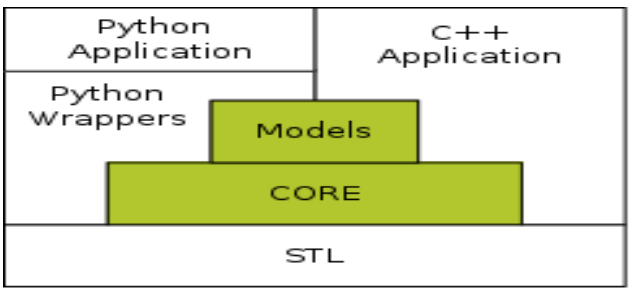
\includegraphics[width=5in]{figures/literature/ns3-architecture}
	\caption[Ns-3 architecture]{\small 
		Ns-3 architecture. Reprinted from \shortciteA{Siraj2012} }
	\label{fig:ns3-architecture}
\end{figure}

\subsection{Robotics Simulator and Robotic Software}

Applications for physical robots can be created using robotics simulator without depending on the real hardware. This saves time and cost in the development of the application. Certain robotics simulator can render 3D model of robots and its environment, and can emulate robotic models, sensors, and control in virtual environment. They use physics engine to make the simulation more realistic.

\shortciteA{Staranowicz2011} has conducted a survey presenting comparison between the popular commercial and open-source robotic software for simulation and interfacing with real robots.  \shortciteA{Ivaldi2014} has conducted an online survey where participants present their feedback about the tools and use of dynamic simulation in robotics.

The most used robotics simulator are:
\begin{itemize}
	\item \textit{Gazebo.} Gazebo can simulate multiple robots in outdoor environments. It supports multiple physics engine. It can intergate with ROS using a set of ROS packages named gazebo\_ros\_pkgs. Gazebo is open source and free to use.
	\item \textit{ODE.} Open Dynamics Engine is a open-source physics library for simulating rigid body dynamics. It is used in computer games and simulation tools. It is open source.
	\item \textit{Bullet.} Bullet is an open-source physics library and is used in 3D animation software and game engines. It is open source.
	\item \textit{V-Rep.} V-Rep is a robot simulator software developed by Coppelia Robotics. It is free for academic usage. Commercial license is not free. 
	\item \textit{Webots.} Webots is an open-source robot simulator developed by Cyberbotics. It was open sourced in 2018. Robots can be modeled, programmed and simulated with the provided development environment.
\end{itemize}  

In this study, I intend to use Gazebo as the robotics simulator because:

\begin{itemize}
	\item The UAV firmware PixHawk provides SITL simulation for Gazebo and is the recommended option. 
	\item Gazebo supports PixHawk provided quad-copter (Iris).
	\item Gazebo supports multiple quad-copters.
	\item External world can be built in Gazebo using real world height maps.
	\item Gazebo supports sensors such as GPS and cameras.
	\item Gazebo can be integrated with ROS.
	\item Gazebo server provides API to integrate with other software. In my use case, I update the FANET nodes in ns-3 using the position provided by the robotics simulator. 
\end{itemize}

\section{Robot Operating System}
\shortciteA{Quigley2009} presents an overview of Robot Operating System (ROS). ROS is a framework for robotics software. It provides set of tools and communication layer on top of a host operating system, which helps in developing software for robotics. Availability of plethora of open source ROS packages avoids reinventing the wheel while developing the application.

ROS provides peer-to-peer connection to different processes of the robotics system. Each process is called a node and handles a specific aspect of the robotic system. The peer-to-peer topology makes use of a master node which enables the running nodes to find each other at run-time. Nodes exchange information with each other using messages. A message is a predefined strictly typed data structure. Nodes can exchange messages using either topic or service.

Nodes can publish message on a topic. Another node which uses the data generated by it can subscribe to the topic to receive messages. Nodes and topics have many-to-many association with each other. A single node can publish and subscribe to many topics and a topic may be published and subscribed by many nodes at once.

For synchronous communication, a node may call a service registered by another node. A node sends a request message to call a service and the node providing the service will reply with a response message. Unlike topics, service of a particular name can only be advertised by one node.

Nodes, topics and services can be grouped into namespaces. Topics and services follow URI reference naming convention. For example a topic that publishes GPS information for UAV 1 in a multi-UAV system may be named as \textit{/uav0/global\_position/gps}.

ROS has tranformation system called tf/tf2. Tf2 is the new iteration of the transformation library. The transformation system helps the user keep track of multiple coordinate frames over time by using a tree structure to maintain relationship between coordinate frames. It allows for easy transformation of data between any two coordinate frames.

ROS has a wide array of tools for creating, debugging, inspecting and visualizing the data exchanged between the different nodes which speeds up the development.


\section{Complete Coverage Problem}



\FloatBarrier


\setlength{\footskip}{8mm}

\chapter{Methodology}
\label{ch:methodology}

\textit{The different components of the proposed system and how they work together are described in this chapter.}

\section{System Overview}
The system will use multiple drones with PixHawk flight controllers, each paired with an individual companion computer and a ground control station (GCS). The operator will set the origin of the global map and select a region of interest on the GCS using Mapviz, a ROS package. The system will then create a grid over the region of interest and calculate paths for the drones. After the expected paths are calculated, the system will calibrate the drones by finding an accurate transformation between each drone's local frame of reference and the global frame. To accomplish this, the drones will move in a predefined flight path while the transformations between each local map of and the global map is refined. After calibration is complete, the system coordinates the flights of the drones as they move along the path the system calculated ensuring coverage of the region of interest. While flying their paths, the drones will stream images from their cameras to the GCS. On the GCS, the SfM module will receive the images and construct an aerial map (a textured 3D mesh) with respect to the global map frame for the region of interest initially selected by the operator.

All the components will be run on a single computer while simulating the system. In simulation mode, PX4 will be run in software in the loop (SITL) mode. Gazebo will be used to visualize the physical world and render simulated video feeds. Network Simulator 3 (NS3) will be used to simulate the networking functions of the wireless mesh network.

\section{System Design}

The different compomenets comprising the system are described here.

\subsection{Components}

The system can be divided into two domains, one comprising the components in the drones, and the other comprising the components in the GCS. Components running on drones will not share information with other drones; they will only share with the GCS. These components will be involved with vehicle platform manipulation and forwarding the video stream. The components on the GCS will be involved with aerial mapping from the video stream received, getting the initial region of interest from the operator, planning the path of each drone, and coordinating the movement of each drone during plan execution.

The flight controller will be installed with PX4 firmware execution. The companion computers and the GCS will run Ubuntu or Raspbian Linux with their Robot Operating System (ROS) installed and will be connected to a wireless mesh network through the IEEE 802.11 devices.

The components on the GCS are:
\begin{itemize}
  \item Robot Operating System: All the components will be designed and implemented with ROS as the base infrastructure. This will give access to the plethora of ROS tools and packages.
  \item Structure from Motion: The aerial map from the video feed of the drones will be constructed by this component.
  \item mapviz: Mapviz is a ROS-based visualization tool with a plug-in system focused on visualization of 2D data. It shows tiled maps using the Microsoft Bing Maps API and has plugins to select polygons on the map, show markers, show NavSat data, among other features that fit the requirements of this system. Mapviz also allows us to fix the origin of the global map.
  \item pegasus\_planner: A new multi-agent path planning ROS node designed for the project.
  \item pegasus\_controller: A new ROS node that will calculate and maintain translations between different map frames, monitor links with the drones, transmit path planning information to the drones, and coordinate the drones during flight.
\end{itemize}

The components in the drones are:
\begin{itemize}
  \item Flight Controller: The drones will use Pixhawk flight controllers with PX4 as their firmware.
  \item Companion Computer: The companion computer will control the flight controller in OFFBOARD mode.
  \item Robot Operating System: The software components will be designed and implemented as ROS nodes.
  \item mavros: The companion computer will use mavros, a ROS package for MavLink communication between companion computers, and flight controllers, to control the flight controller in OFFBOARD.
  \item pegasus\_commander: A new ROS node designed for the project that receives paths and control messages from the GCS. It will also send local poses, GPS positions, flight controller status updates, and GCS link monitoring information.
  \item video streamer: The video feed from the onboard camera will be captured and streamed to the GCS by this component.
\end{itemize}

Figure \ref{fig:system-overview} illustrates the different components of the system controlling three drones.

\begin{figure} \label{fig:system-overview}
  \centering
  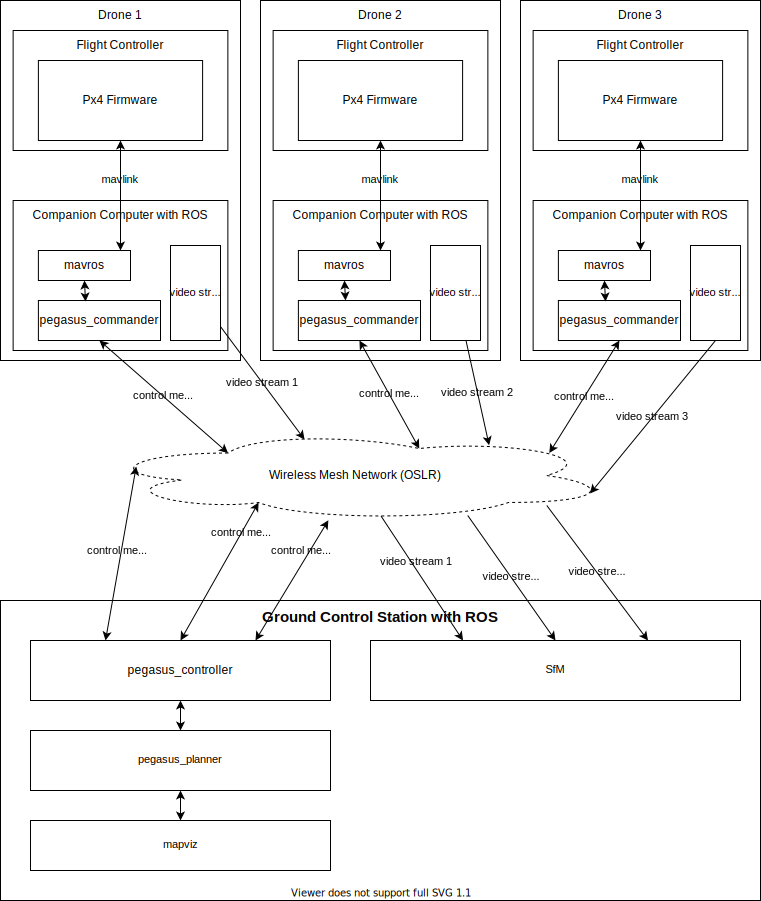
\includegraphics[width=5in]{figures/methodology/system-overview}
  \caption[Pegasus System Overview]{\small Pegasus system overview with three drones.}
\end{figure}


The operator will select the global map origin and region of interest through mapviz. The pegasus\_planner will create a grid-based representation of the region of interest and plan the paths for the drones in the global map reference frame. The initial position of each drone will be provided by pegasus\_controller  to pegasus\_planner. The path planned by pegasus\_planner will be sent to pegasus\_controller. Pegasus\_controller will run a calibration routine on each of the drones to find the transformation between the local origin of the drone and the global map origin. After calibration completes, pegasus\_controller will transform the paths for the drones from global map to the local map for each drone and send it to the drone. Pegasus\_controller will monitor the link with each drone by sending a periodic heart-beat packet. If a drone does not receive a heart-beat packet for some interval, it will change to Return To Home (RTL) mode and abort its current path. To avoid collision, pegasus\_controller will also maintain a path index counter. Paths are made up of a list of poses. Pegasus\_controller will tell each drone to move to the next pose in its path when all the drones have reached their current goal pose.

The SfM module will receive image streams from the drones, and construct an aerial map with respect to the global map frame for the region of interest selected by the operator.

The drones will use mavros, which exposes MavLink protocol parameters and services as ROS topics and services. Pegasus\_commander will receive commands and path information from the GCS and execute its plan while sending local poses, global GPS positions, and flight controller state information back to the GCS. The video streamer will capture images from the onboard camera, apply GPS tags and send them to the GCS.

\subsection{Ground Control Station}

The GCS will be a computer running Ubuntu, with ROS installed. In my particular case, the GCS has an i7 processor, 16 GB of RAM, and a wireless LAN interface.

\subsubsection{Mapviz}
Mapviz requires the operator to select the global map origin as a ROS parameter. ROS parameters can be set through the rosparams command-line tool, programmatically or in the launch file. In our case, we set the local map origin though the launch file using the ROS package swri\_transform\_util.

\begin{verbatim}
<?xml version="1.0"?>
<launch>
  <node pkg="mapviz" type="mapviz" name="mapviz"></node>
  <node pkg="swri_transform_util" type="initialize_origin.py"
    name="initialize_origin" >
    <param name="local_xy_frame" value="/map"/>
    <param name="local_xy_origin" value="control_station"/>
    <rosparam param="local_xy_origins">
      [{
        name: control_station,
        latitude: 14.081104,
        longitude: 100.612743,
        altitude: 7,
        heading: 0.0
      }]
    </rosparam>
  </node>
</launch>
\end{verbatim}

\begin{figure} \label{fig:mapviz-screenshot}
  \centering
  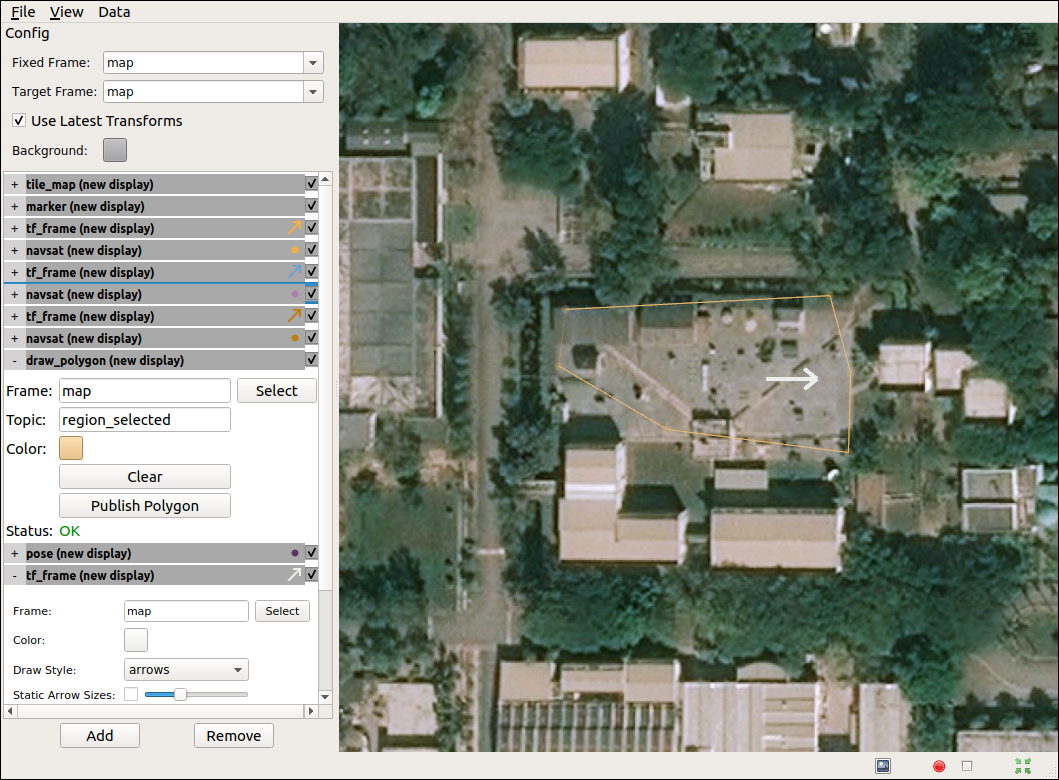
\includegraphics[width=5in]{figures/methodology/gcs/mapviz/screenshot}
  \caption[Mapviz visualizer]{\small Mapviz visualizer with origin set near CSIM.}
\end{figure}

It will publish two ROS topics:
\begin{itemize}
  \item /local\_xy\_origin: Origin of the global map.
  \item /mapviz/region\_selected: The points of the polygon as selected by the user.
\end{itemize}

\subsubsection{Pegasus\_planner}

Pegasus\_planner will handle the following tasks:
\begin{itemize}
  \item Generate grid cells in the region of interest.
  \item Try to calculate the optimal paths for each drone, such that they avoid collisions and stay within the constraints of the wireless mesh network in the global map frame.
\end{itemize}

To generate a valid grid inside the region of interest, consider a polygon with $n$ vertices:

\begin{figure} \label{fig:pegasus-planner-generate-grid-polygon}
  \centering
  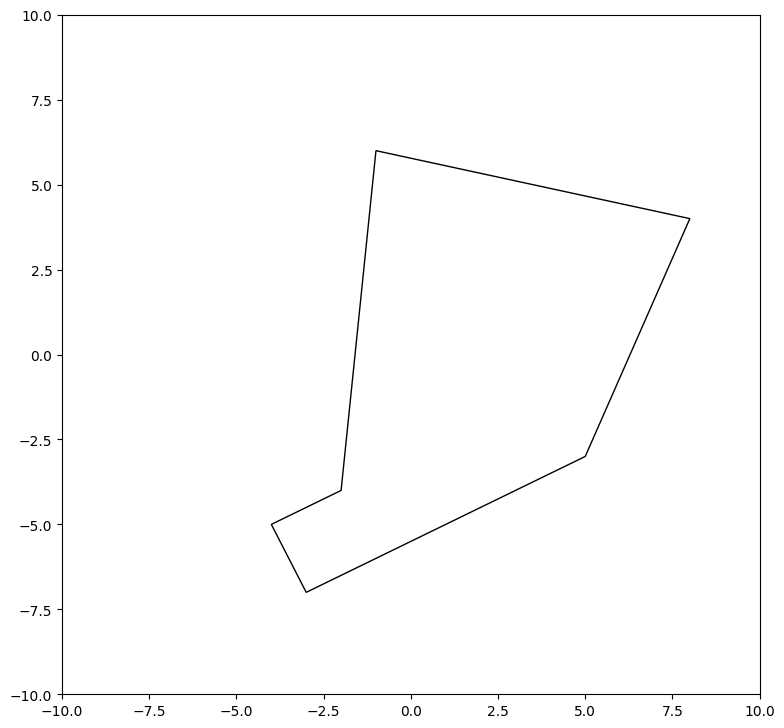
\includegraphics[width=4in]{figures/methodology/pegasus_planner/generate_grid/polygon}
  \caption[Polygon Showing the Area of Interest]{\small Polygon showing the area of interest.}
\end{figure}

$$
\text{polygon} = \begin{bmatrix}
  x^0 & y^0 \\
  x^1 & y^1 \\
  x^3 & y^2 \\
  \vdots  & \vdots \\
  x^{n-1} & y^{n-1} \\
\end{bmatrix}. 
$$

The vertices are arranged counter-clockwise/clockwise. To find the bounding box of the polygon, we need to find the vertices.

$$
\text{boundingBox} = \begin{bmatrix}
  x_{min} & y_{min} \\
  x_{max} & y_{min} \\
  x_{max} & y_{max} \\
  x_{min} & y_{max}
\end{bmatrix},
$$

\begin{figure} \label{fig:pegasus-planner-generate-grid-bounding-box}
  \centering
  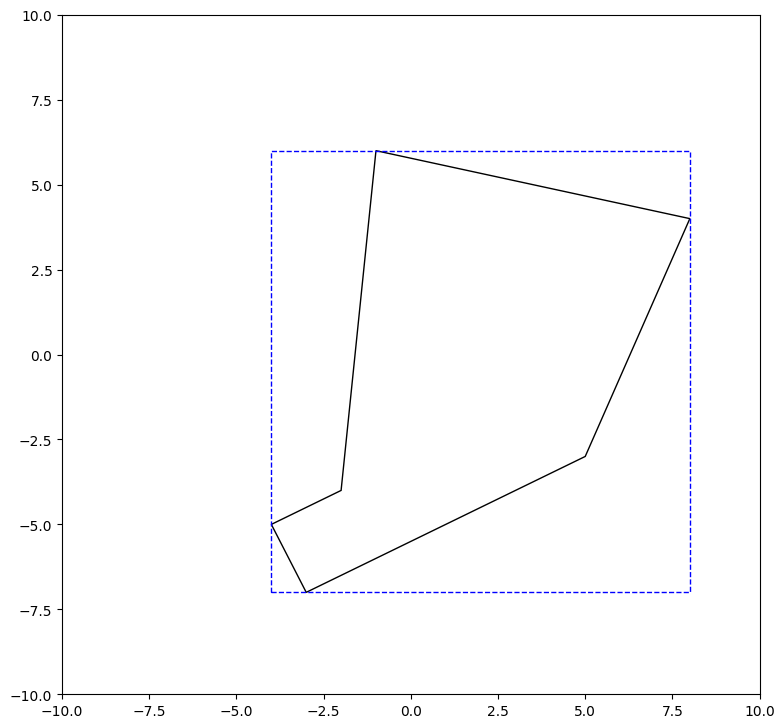
\includegraphics[width=4in]{figures/methodology/pegasus_planner/generate_grid/bounding-box}
  \caption[Bounding Box on the Polygon Showing the Area of Interest]{\small Bounding box on the Polygon showing the area of interest.}
\end{figure}

where each row defines a vertex. Consider a grid with $n$ cells either horizontally or vertically. Let $c$ be the grid cell size.

$$c = \text{BoundingBox}_{width|heigh} \div  n $$

Alternatively, we can set a fixed size for each cell, or calculate the cell size from camera parameters and the altitude of the drone.

We can then calculate the coordinates $(b^{i,j}_x, b^{i,j}_y)$ of the bottom left vertex of each cell.

$$\text{cells} =\begin{bmatrix}
  b^{0,0}_x & b^{0,0}_y \\
  b^{1,0}_x & b^{1,0}_y \\
  b^{2,0}_x & b^{2,0}_y \\
  \vdots & \vdots \\
  b^{i_{max} - 1,0}_x & b^{i_{max} - 1,0}_y \\
  b^{0,1}_x & b^{0,1}_y \\
  b^{1,1}_x & b^{1,1}_y \\
  b^{2,1}_x & b^{2,1}_y \\
  \vdots & \vdots \\
  b^{i_{max} - 1,0}_x & b^{i_{max} - 1,0}_y \\
  \vdots & \vdots \\
  b^{i_{max} - 1,j_{max}-1}_x & b^{i_{max} - 1,j_{max} - 1}_y \\
\end{bmatrix}$$

$$b^{i,j}_x = x_{min} + i * c$$
$$b^{i,j}_y = y_{min} + j * c$$

$i$, $j$ are the index in $x$  and $y$ axis respectively.


We can get the range of $i$ and $j$ as follows.
$$i_{max} = \left\lceil\frac{x_{max} - x_{min}}{c}\right\rceil $$
$$j_{max} = \left\lceil\frac{y_{max} - y_{min}}{c}\right\rceil$$

Let the number of vertices in $gridCells$ be $k$:
$$ k = i_{max} \times j_{max}.$$


We can then calculate grid index $(i,j)$ from $[0, k]$:

$$j = \left\lfloor\frac{k}{i_{max}}\right\rfloor$$
$$i = k  - j \times i_{max}.$$

\begin{figure} \label{fig:pegasus-planner-generate-cells}
  \centering
  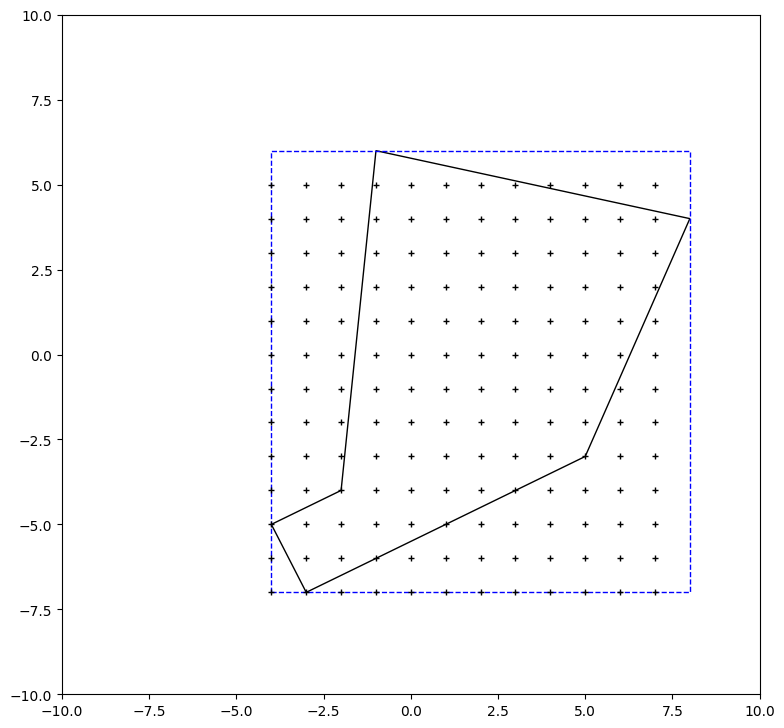
\includegraphics[width=4in]{figures/methodology/pegasus_planner/generate_grid/cells}
  \caption[Cells in the Bounding Box]{\small Bottom left position of the cells in the bounding box.}
\end{figure}

Since the vertex $v$ of the polygon is arranged counter-clockwise/clockwise, we can easily get the vertices of line segment for each side of the polygon.

$$v_i = (x_i, y_i)$$
$$s < n$$

$$\text{polygonLineSegments}=\begin{bmatrix}
  v_0 & v_1 \\
  v_1 & v_2 \\
  \vdots & \vdots \\
  v_s & v_{s+1} \\
  \vdots & \vdots \\
  v_{s_{max}-1} & s_0 \\
\end{bmatrix}$$

$$=\begin{bmatrix}
  x_0 & y_0 & x_1 & y_1 \\
  x_1 & y_1 & x_2 & y_2\\
  \vdots && \vdots \\
  x_s & y_s & x_{s+1} & y_{s+1} \\
  \vdots && \vdots \\
  x_{n-1} & y_{n-1} & x_{0} & y_{0} \\
\end{bmatrix}$$

We can imagine that the center of each grid cell projects a line parallel to the $x$ axis till $x_{max} + 1$.

$$\text{cellCenter} = [\text{cells}] +  \frac{c}{2}$$
$$\text{rays} = \begin{bmatrix}
  \text{cellCenter}_x^{0,0} & \text{cellCenter}_y^{0,1} & x_{max} + 1 & \text{cellCenter}_y^{0,1} \\
  \text{cellCenter}_x^{1,0} & \text{cellCenter}_y^{1,1} & x_{max} + 1 & \text{cellCenter}_y^{1,1} \\
  \text{cellCenter}_x^{2,0} & \text{cellCenter}_y^{2,1} & x_{max} + 1 & \text{cellCenter}_y^{2,1} \\
  \vdots && \vdots \\
  \text{cellCenter}_x^{k-1,0} & \text{cellCenter}_y^{k-1,1} & x_{max} + 1 & \text{cellCenter}_y^{k-1,1} \\
\end{bmatrix}
$$
\begin{figure} \label{fig:pegasus-planner-generate-ray}
  \centering
  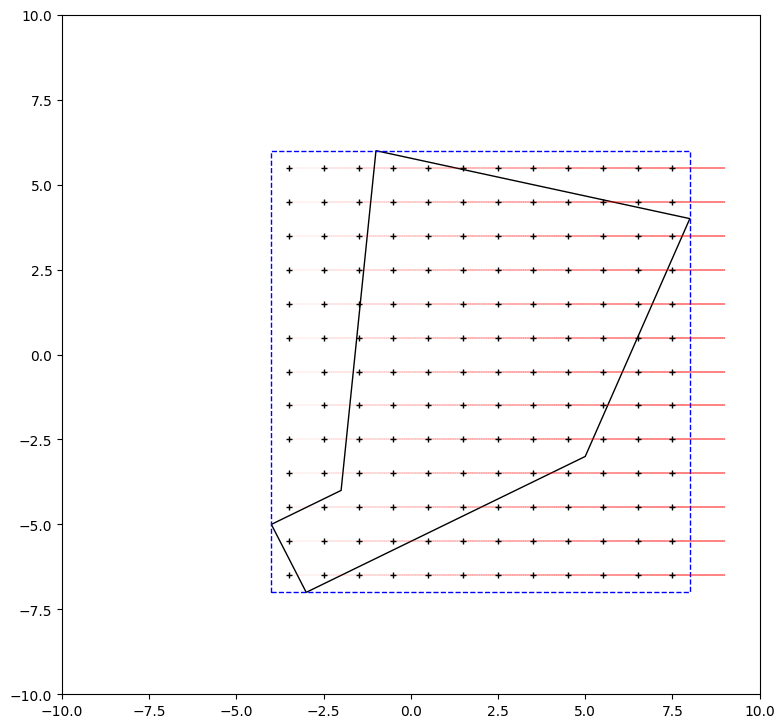
\includegraphics[width=4in]{figures/methodology/pegasus_planner/generate_grid/ray}
  \caption[Rays projecting from cell centre to $x_{max} + 1$]{\small Rays projecting from cell centre to $x_{max} + 1$.}
\end{figure}

Now we apply ray tracing to check if $cell^{i,j}$ is inside our polygon or not. We count how many intersections each $rays^{i,j}$ makes with all the lines in $polygonLineSegments$. If the number of intersections are even, then the $cell$ is outside the polygon. If the number of intersections are odd, then the $cell$ is inside the polygon. We now have the valid cells that can the drones can traverse.
\begin{figure} \label{fig:pegasus-planner-generate-valid-cells}
  \centering
  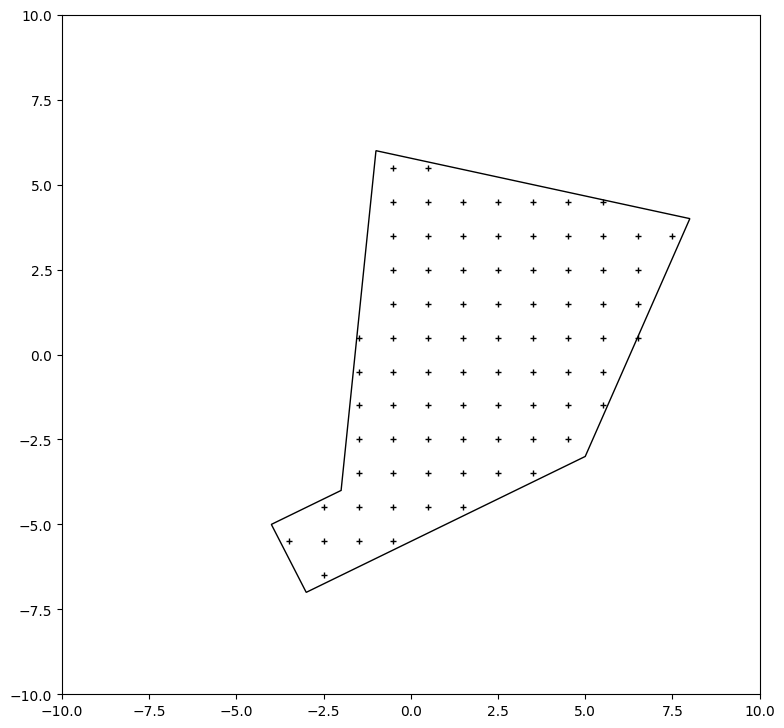
\includegraphics[width=4in]{figures/methodology/pegasus_planner/generate_grid/valid-cells}
  \caption[Grid inside the region of interest]{\small Grid cells inside the region of interest.}
\end{figure}

To plan the path for the drones.....

\subsubsection{Pegasus\_controller}

Pegasus\_controller will be responsible for:
\begin{itemize}
  \item Calculating and maintaining the transformations between the local map frames of each drone and the global map frame.
  \item Coordinating and sending control messages to the drones. Refer to section \ref{section:pegasus-commander} for the list of control messages available.
  \item Monitoring the link with the drones by sending heart beat control message.
  \item Publishing local pose, global GPS coordinates and state of each drone, received from pegasus\_commander as ROS topics.
  \item Publishing the transposed pose and transposed GPS position of all the drones in global map frame.
\end{itemize}

It will have the following states:
\begin{itemize}
  \item IDLE: It will not do anything.
  \item OFFBOARD\_MODE: It will send SET\_OFFBOARD control message to the drones and wait for confirmation.
  \item ARMING: It will send SET\_ARM control message to the drones and wait for confirmation.
  \item TAKE\_OFF: It will send TAKEOFF control message with the altitude to the drones.
  \item CALIBRATE: It will send the calibration path to the drones and coordinate the flight of the drone along the calibration path. It will also capture the corresponding local poses and global GPS positions for calculation the map transformations.
  \item GENERATE\_TRANSFORMS: It will generate the transforms between the local map frame of each drone and the global map frame using the corresponding points collected in CALIBRATE state.
  \item RUN: It will transform the path published by pegasus\_planner on ROS topic /pegasus/[agent]/path to each drone local frame, send it to the drones using SET\_PATH control message, and coordinate the drones using GOTO\_PATH\_INDEX control message.
  \item COMPLETE: It will reach this state when the system's execution is complete. Set the drone to Return mode by sending SET\_RTH control message.
\end{itemize}

Algorithm \ref{find-transforms} will be used to find transforms between local map of each drone and the global map.

\renewcommand{\algorithmicrequire}{\textbf{Input:}}
\renewcommand{\algorithmicensure}{\textbf{Output:}}
\renewcommand{\algorithmicforall}{\textbf{for each}}
\begin{algorithm}
  \caption{Find Local To Global Transformation}
  \label{find-transforms}
  \begin{algorithmic}
    \REQUIRE $L$: set of all corresponding local poses
    \REQUIRE $G$: set of all corresponding global GPS positions
    \REQUIRE $O$: global map origin GPS coordinate
    \ENSURE $T$: transformation between local and global map
    \STATE $\widetilde{O} \gets \textsc{Convert-to-UTM}(O)$
    \STATE $\widetilde{G} \gets \textsc{Convert-to-UTM}(G)$
    \STATE $M \gets \widetilde{O} - \widetilde{G}$
    \STATE $\widehat{M} \gets \textsc{Remove-Z-axis}(\widetilde{M})$
    \STATE $\widehat{L} \gets \textsc{Remove-Z-axis}(L)$
    \STATE $H \gets \textsc{Find-Homography}(\widehat{L}, \widehat{M}, \text{RANSAC})$
    \STATE $T \gets \begin{bmatrix}
      H_{1,1} & H_{2,1} & 0 & H_{3,1} \\
      H_{1,2} & H_{2,2} & 0 & H_{3,2} \\
      0 & 0 & 1 & 0 \\
      0 & 0 & 0 & 1
    \end{bmatrix}$

  \end{algorithmic}
\end{algorithm}

\subsection{Drone}

\subsubsection{PX4}
The drone runs PX4 Firmware on the flight controller. The flight controller's movement and altitude can be controlled in Offboard mode through the MAVlink protocol. This mode supports only a very limited set of MAVLink commands.

MAVLink commands supported in Offboard modes are:
\begin{itemize}
  \item SET\_POSITION\_TARGET\_LOCAL\_NED: Control vehicle position.
  \item SET\_ATTITUDE\_TARGET: Control vehicle altitude and orientation.
\end{itemize}

PX4 supports the coordinate frames (coordinate\_frame field): MAV\_FRAME\_LOCAL\_NED and MAV\_FRAME\_BODY\_NED.

A stream of setpoint commands must be received by the vehicle prior to engaging the mode, and in order to remain in the mode (if the message rate falls below 2Hz the vehicle will stop). In order to hold position while in this mode, the vehicle must receive a stream of setpoints for the current position.

Offboard mode requires an active connection to a remote MAVLink system (e.g. companion computer or GCS). If the connection is lost, after a timeout (COM\_OF\_LOSS\_T) the vehicle will attempt to land or perform some other failsafe action. The action is defined in the parameters COM\_OBL\_ACT and COM\_OBL\_RC\_ACT which can be set through mavros' mavparam.

\subsubsection{Mavros}

Mavros is a ROS node that provides ROS interfaces for communication with various autopilots with MAVLink communication protocol.
The ROS services provided by Mavros,  of interest for this system are:
\begin{itemize}
  \item mavros/set\_mode: Required to set mode of the flight controller to Offboard mode.
  \item mavros/cmd/arming: Required to arm the flight controller.
\end{itemize}

The ROS topics published by Mavros, useful for this system are:
\begin{itemize}
  \item mavros/state: Publishes the state of the flight controller.
  \item mavros/local\_position/pose: Publishes pose, i.e. position and orientation of the flight controller in the local frame. Mavros handles the translation between NED and ENU conventions.
  \item mavros/global\_position/global: Publishes the GPS coordinates, i.e. latitude, longitude and altitude of the flight controller.
\end{itemize}

The ROS topics subscribed by Mavros, that this system will use are:
\begin{itemize}
  \item mavros/setpoint\_position/local: Set the pose, i.e. position and orientation that the flight controller is desired to achieve in local frame.
\end{itemize}

\subsubsection{Pegasus\_commander} \label{section:pegasus-commander}

Pegasus\_commander is a new ROS node, customized for this study that uses the topics and services provided by mavros to control the drone in Offboard mode. It receives control messages from the GCS. It also monitors the link between GCS and the drone, and a heart beat control message is not received for a particular duration, then the flight controller is set to Return mode.

The different types of control messages that will be received by pegasus\_commander from GCS are:
\begin{itemize}
  \item HEART\_BEAT: GCS heart beat in regular intervals.
  \item SET\_OFFBOARD: Put the flight controller in Offboard mode.
  \item SET\_RTH: Put the flight controller in Return mode.
  \item SET\_ARM: Arm the flight controller.
  \item TAKEOFF(float): Set the altitude of the drone.
  \item SET\_PATH(pose): Set the path that the drone needs to follow in local map frame.
  \item GOTO\_PATH\_INDEX(int): Set the local position to the pose in the given index.
\end{itemize}

The different types of control messages that will be sent to the GCS are:
\begin{itemize}
  \item HEART\_BEAT\_ACK: Acknowledgment to the GCS's heart beat.
  \item PATH\_INDEX\_REACHED(int, pose): Return the path index and the local pose when the drone reaches the set-point indicated with GOTO\_PATH\_INDEX message from GPS.
  \item SUCCESS(message): Return success confirmation for message from GCS.
  \item FAILED(message): Return fail confirmation for message from GCS.
\end{itemize}

Pegasus\_commander also transmits the state, local pose and GPS coordinated of the drone to the GCS in regular intervals.

\subsubsection{Video Streamer}

The images from the onboard camera of the drone will be captured. Then each image frame will be geo-tagged with the current GPS coordinates from the flight controller and the geo-tagged image feed will be streamed to the GCS.

\subsection{Simulation}

Most of the components will remain the same regardless of whether runnng in simulation or in the real world. The simulation will run in a single computer. Three more components will be utilized to simulate the system:
\begin{itemize}
  \item Gazebo: Gazebo simulator will be used because it supports fleet of drones and camera feed.
  \item Network Simulator 3: NS3 will be used to simulate the wireless mesh network functions.
  \item pegasus-net-sim: A custom NS3 module that will simulate the mobility of the dro\textsc{}nes and push and pop actual control messages and video feed between the drones and the GCS through the simulator. It will also publish the status of each device in the network.
  \item pegasus\_networl\_status\_util\_node: A custom ROS node that will receive noise and signal strength from pegasus-net-sim and publish the signal-to-noise ratio (SNR) value of each drone as ROS topic.
\end{itemize}

\begin{figure} \label{fig:system-simulation-overview}
  \centering
  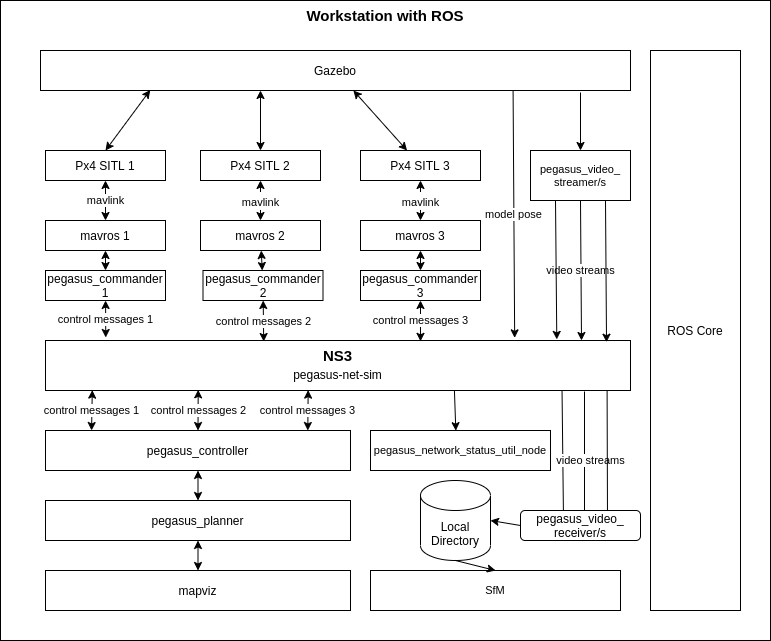
\includegraphics[width=5in]{figures/methodology/system-simulation-overview}
  \caption[Pegasus Simulation System Overview]{\small Pegasus Simulation System Overview}
\end{figure}

Figure \ref{fig:system-simulation-overview} describes the simulation system schematically.

Gazebo will be used to simulate the world, the drone mechanics and the video feed. Pegasus-net-sim, a Network Simulator 3 custom module will be used to simulate the wireless mesh network. Pegasus-net-sim will receive the model info from Gazebo and update the position of its nodes. Each node in pegasus-net-sim will have NS3PegasusApp, a custom NS3 application installed, which will send and receive packets in the simulated network. Pegasus-net-sim will function as a proxy application that will receive data in one UDP port, simulate it in NS3 and transmit it through another UDP socket. Using the trace feature in NS3, pegasus-net-sim will publish the noise and signal value for each node of the wireless mesh network.

\FloatBarrier

\setlength{\footskip}{8mm}

\chapter{Experimental Results}
\label{ch:results}

\textit{Some intro..}


\FloatBarrier


\setlength{\footskip}{8mm}

\chapter{Conclusion and Recommendations}
\label{ch:conclusion}

\textit{Some text..}

\FloatBarrier



% NEED TO CHANGE THE SECTION NUMBER FOR REFERENCES ACCORDINGLY.
\addcontentsline{toc}{chapter}{6 \hskip 3.55em References}

\bibliographystyle{apacite}
\bibliography{references}

% COMMENT THE LINES ABOUT APPENDICS OUT IF YOU DO NOT HAVE THIS SECTION.

%%%%%%%%%%%%%%%%%%%%%%%%%%%%%%%%%%%%%%%%%%%%%%%%%%%%%%%%%%%%%%%%%%%
%                                                                 %
%                            APPENDICES                           %
%                                                                 %
%%%%%%%%%%%%%%%%%%%%%%%%%%%%%%%%%%%%%%%%%%%%%%%%%%%%%%%%%%%%%%%%%%%
\newpage\pagestyle{plain}
\theappendix

% NEED TO CHANGE THE SECTION NUMBER FOR REFERENCES ACCORDINGLY.
\addcontentsline{toc}{chapter}{7 \hskip 3.55em Appendices}

\setlength{\footskip}{8mm}

% NOTE: NEED TO DO EVERYTHING SUCH AS SECTION NUMBER OR FIGURE NUMBER 
% MANUALLY IN THIS CHAPTER.

\renewcommand{\thefigure}{A.\arabic{figure}}

\begin{center}
{\large \bf Appendix A\\ \vskip 1em .. TITLE HERE ..\\ \vskip 1em}
\vskip 1em
\end{center}

\FloatBarrier

\singlespace
 
{\bf Section Name} \\ 

Figure~\ref{fig:monitoring-test} shows something. 

Some text ..

\begin{figure}[t]
  \centering
  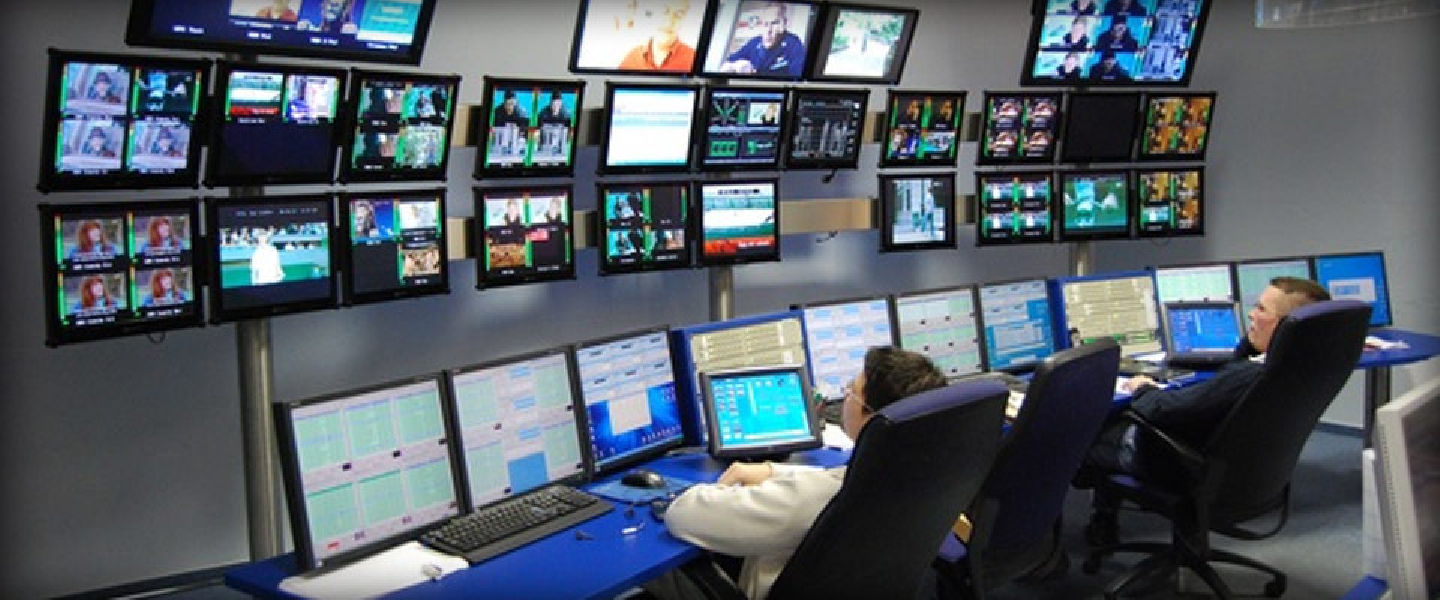
\includegraphics[width=5in]{figures/monitoring}
  \caption[]{\small CCTV monitoring
    room. Reprinted from the Twenty First Security Web site
    (\url{http://www.twentyfirstsecurity.com.au/}).}
  \label{fig:monitoring-test}
\end{figure}

\FloatBarrier



\end{document}
